\section{Introduction}

In this chapter, we propose a numerical method to solve the governing equations derived previously for a compressible active nematic gel.  The governing Eqs.~(\ref{eq_box_A_1}-\ref{eq_box_A_7}) of the proposed model are non-linear and tightly couple nematic, velocity and density fields. Similar models are usually approximated numerically with  Lattice Boltzmann \cite{marenduzzo2007,cates2009} or Hybrid Boltzmann  \cite{desplat2001} methods, for which a freely available  implementation is available (\href{https://github.com/ludwig-cf/ludwig}{the Ludwig code}). The solution of the governing equations has also been approximated using finite element methods \cite{goudiaby2021,becker2008, norton2018}. Our finite element computational approach builds on the variational Onsager's formalism, which makes numerical discretization straightforward by simply performing extremization of the Lagrangian in a constrained functional space given by the finite element approximation of the process variable fields. For time discretization, we resort to the  implicit Euler method. We apply  this numerical method to study the active self-organization around a wound in an active gel, simulating wound healing in large egg cells \cite{benink2000,mandato2001}, and in confined populations of elongated cells \cite{duclos2014}.


%In the Lattice Boltzman algorithm,  first, the individual distribution functions for the velocity and the nematic order are selected on nodes of a lattice. In a second step, the physical variables are mapped in terms of the moments of the distribution functions. In a third step, the distribution functions on each node are updated based on their advection in direction of the neighboring nodes interactions are a result of a collision with density functions at neighbors. These interactions are characterized by collision operators that are formulated such that the original governing equations are recovered.  In the last step, the distribution functions are streamed to the new location. In the hybrid Boltzmann algorithm, the hydrodynamic and incompressible equations are solved with the classic Lattice Boltzman algorithm, and the q-tensor dynamic equation is solved with the finite difference method  
%One of the implementations of the Lattice Boltzmann algorithm for complex fluids, \href{https://github.com/ludwig-cf/ludwig}{the Ludwig code}, based on \cite{desplat2001} is freely available.




\section{Space and time discretization}

In Eqs.~(\ref{eq:Rayleighian}) and~(\ref{eq:Lagrangian}) we expressed the Rayleghian and the Lagrangian in terms of the independent variables $\dot{\rho},\widehat{\bm{q}},\bm{v},\bm{d},\bm{w}$ and $\bm{\zeta}$ to facilitate the derivation of the strong form in the most meaningful way from a physical perspective. However, for numerical purposes, it is more convenient to  consider $\partial_t{\bm{q}}$ and $\bm{v}$ as the sole process variables, with $\widehat{\bm{q}},\bm{d},\bm{w}$ and $\bm{\zeta}$ as derived fields and balance of mass as a strong constraint. From the first line in Eq.~(\ref{eq:change_of_free_energy}), applying the chain rule to compute $\partial_t f$ and using Eq.~(\ref{eq:balance_mass}), we can express the rate of change of the free energy as
\begin{align} \label{eq:discrete_free_energy}
	\dot{\mathcal{F}}\left[\partial_t\bm{q},\bm{v};\rho,\bm{q}\right] = &  \underset{A}{\int} \left\{ \rho \frac{\partial f}{\partial \bm{q}} : \partial_t \bm{q} + \left(\rho \frac{\partial f}{\partial \nabla \bm{q}}\right) \cdddot \, \nabla \partial_t \bm{q} + f \left[r-\nabla\cdot\left(\rho\bm{v}\right)\right] \right\}dA  \\ &  +  \underset{\partial_{N}A}{\int} f\rho \bm{v} \cdot\bm{N} dl. \nonumber
\end{align}
For the dissipation and power potentials, we directly substitute the definitions of $\bm{w}$ and $\bm{\zeta}$ as a function of gradients of $\bm{v}$ and we use Eq.~(\ref{eq:Jaumann}) to write $\widehat{\bm{q}}$ in terms of $\partial_t \bm{q}$ and $\bm{v}$, formally leading to functionals of the form $\mathcal{D}[\partial_t\bm{q},\bm{v};\rho,\bm{q}]$ and $\mathcal{P}[\partial_t\bm{q},\bm{v};\rho,\bm{q}]$.
%\begin{align}   \label{eq:discrete_dissipation}
%	\mathcal{D}[\partial_t\bm{q},\bm{v};\rho,\bm{q}] = \underset{A}{\int} d\left(\partial_t\bm{q},\bm{v};\bm{q}\right)  \rho dA,
%\end{align}
%\begin{align}  \label{eq:discrete_power}
%	\mathcal{P}[\partial_t\bm{q},\bm{v};\rho,\bm{q}] = \underset{A}{\int} p\left(\partial_t\bm{q},\bm{v};\bm{q}\right)  \rho dA.
%\end{align}
Combining these functionals,  the Rayleighian can be expressed as
\begin{align}  \label{eq:ray_discrte}
	\mathcal{R}[\partial_t\bm{q},\bm{v};\rho,\bm{q}] = \dot{\mathcal{F}}[\partial_t\bm{q},\bm{v};\rho,\bm{q}]+ \mathcal{D}[\partial_t\bm{q},\bm{v};\rho,\bm{q}]+ \mathcal{P}[\partial_t\bm{q},\bm{v};\rho,\bm{q}].
\end{align}
Onsager's formalism then provides an alternative form of the governing equations by minimizing this Rayleighian with respect to $\partial_t \bm{q}$ and $\bm{v}$.  We describe here the weak formulation of the governing equations in Eulerian form, but the framework can be easily adapted to Lagrangian formulations. Minimization with respect to  $\partial_t\bm{q}$ leads to
\begin{align}
	\label{eq:weak_q_disc}
	0=\delta_{\partial_t \bm{q}} \mathcal{R}=  \underset{A}{\int}  \bigg[ \left(\frac{\partial  f}{\partial \bm{q}} +   \frac{\partial d}{\partial \widehat{\bm{q}}} +  \frac{\partial p}{\partial \widehat{\bm{q}}} \right):\bm{p} + \frac{\partial f}{\partial \nabla \bm{q}} \cdddot \, \nabla \bm{p} \bigg]\rho dA -   \int_{\partial_{N_{\bm{L}}}A} \bm{L}:\bm{p} dl, 
\end{align}
where $\bm{p}$ is an arbitrary variation of $\partial_t \bm{q}$, and hence a traceless and symmetric second order tensor. Note that this equation encodes the same physics as  Eq.~(\ref{eq:var_q}), but takes a different form since there we took variations of $ \widehat{{\bm{q}}}$, which are related to those of $\partial_t \bm{q}$ but are different.  Here, we do not integrate by parts this equation because our objective is to obtain the weak form of the problem to discretize it using a finite element method and not obtain a strong form of the equations. 

Minimization with respect to $\bm{v}$ leads to 
\begin{equation}
	\label{eq:weak_v_disc}
	\begin{aligned}
		\bm{0}=\delta_{\bm{v}} \mathcal{R}=   &~\underset{ A}{\int} \bigg \{-\frac{ f}{\rho} \nabla \cdot \left(\rho\bm{u}\right) + \frac{\partial ( d+ p)}{\partial \bm{v}} \cdot\bm{u} + \left[\frac{\partial ( d+ p)}{\partial \bm{d}} + \frac{\partial ( d+ p)}{\partial \bm{w}}\right] : \nabla\bm{u}   \\ & +   
		\frac{\partial ( d+ p)}{\partial \bm{\zeta}} \cdddot \, \nabla\nabla\bm{u} + \frac{\partial ( d+ p)}{\partial \widehat{\bm{q}}} : \delta_{\bm{v}} \widehat{\bm{q}} \bigg \} \rho dA \\
		&  +   \int_{\partial_{N_{\bm{t}}} A} \big\{(f\rho \bm{N} + \bm{t}) \cdot\bm{u} +  \bm{L} : \delta_{\bm{v}} \widehat{\bm{q}}  + \bm{\Gamma}:\nabla\bm{u}  \big\}dl,
	\end{aligned}
\end{equation}
where $\bm{u}$ is an arbitrary variation of $\bm{v}$. The variation of Jaumann derivative of the nematic order tensor with respect to velocity is given by $\delta_{\bm{v}} \widehat{\bm{q}}=  \nabla\bm{q}\cdot\bm{u} + \frac{1}{2}\left(\bm{q} \bm{\epsilon} -\bm{\epsilon}\bm{q} \right) (\bm{\epsilon}:\nabla\bm{u})$. We note that although Eq.~(\ref{eq:weak_v_disc}) looks different to Eq.~(\ref{eq:weak_v}), both equations lead to the same strong form when combined with Eq.~(\ref{eq:balance_q}), see Section~\ref{equivalence}. For balance of mass, we consider the weak form of Eq.~(\ref{eq:balance_mass}), that is, we multiply this equation by an arbitrary test function $\delta\rho$, integrate, and apply the divergence theorem to the diffusive term to obtain
\begin{equation}
	\label{eq:weak_mass}
	\int_A \left \{\left( \dot{\rho}  + \rho \nabla\cdot\bm{v} - k_p  +\rho k_d\right) \delta \rho  + D\nabla \rho \cdot \nabla \delta \rho \right \} dA \nonumber\\
-  \int_{\partial A} D  \nabla \rho \cdot \bm{N} \delta \rho  dl  = 0.
\end{equation}
We first discretize fields in space following a typical finite element setting based on a mesh with $N$ vertices. Each vertex or node $I$ of the mesh has an associated basis function $B_I(\bm{x})$. The choice of the type of basis function is not trivial in general, as e.g. Eq.~(\ref{eq:weak_v_disc}) contains higher-order derivatives of $\bm{u}$ that would require basis functions with at least square-integrable second order derivatives. We note however, that for $\partial ( d+ p) / \partial \bm{\zeta} = \bm{0}$, as is the case in the present model, only first order derivatives of $\bm{u}$ (and $\bm{v}$) appear, and hence a conventional finite element discretization with $C^0$ continuity can be used. A field, e.g.~$\rho(t)$, is discretized as
\begin{equation}
	\rho(\bm{x},t) = \sum_{I=1}^N \rho_I(t) B_I(\bm{x}),
\end{equation}
where $\rho_I(t)$ is the value of $\rho$ at node $I$ and time $t$. Analogously, we have 
\begin{equation}
	\bm{v}(\bm{x},t) = \sum_{I=1}^N\bm{v}_I(t) B_I(\bm{x}),
\end{equation}
where the nodal degrees of freedom are vectors. 
We represent $\bm{q}(\bm{x},t)$ as
\begin{equation}
	\bm{q}(\bm{x},t) = \begin{pmatrix}
		q_1(\bm{x},t) & q_2(\bm{x},t)\\
		q_2(\bm{x},t) & -q_1(\bm{x},t)
	\end{pmatrix},
\end{equation}
and discretize its components as
\begin{equation}
	q_1(\bm{x},t) = \sum_{I=1}^N q_{1I} (t) B_I(\bm{x}), \qquad  q_2(\bm{x},t) = \sum_{I=1}^N q_{2I} (t) B_I(\bm{x}).
\end{equation}
Thus, we have 5 degrees of freedom per node, namely $\rho_I, v_{1I}, v_{2I}, q_{1I}$ and $q_{2I}$.

To discretize Eq.~(\ref{eq:weak_q_disc}), we express variations $\bm{p}$ as linear combinations of the following traceless symmetric tensors 
\begin{equation}
	\begin{pmatrix}
		B_I(\bm{x}) & 0\\
		0 & -B_I(\bm{x})
	\end{pmatrix} \qquad \mbox{and} \qquad  \begin{pmatrix}
		0 & B_I(\bm{x})\\
		B_I(\bm{x}) & 0
	\end{pmatrix},
\end{equation}
for all $I$.  Using the space-discretized nematic tensor and the variations defined above, the discretized form of balance of generalized force conjugate to nematic order in Eq.~(\ref{eq:weak_q_disc}) becomes a set of $2N$  equations of the form 
\begin{align} \label{eq_week_1}
	\underset{A}{\int}  & \bigg\{ \bigg[ 	 \eta_{\rm rot} \widehat{q}_1 +  \frac{1}{2} \beta \left(\nabla_1 v_1 - \nabla_2 v_2 \right)+ \left(2a+bS^{2} \right)q_1 - \rho \lambda_{\bigodot} q_1 \bigg]B_I  \\ & +  
	L  \bigg(\nabla_1 B_I \nabla_1 q_1  \nonumber  +   \nabla_2 B_I \nabla_2 q_1 \bigg) \bigg \}   d A + \int_{\partial_{N_{\bm{L}}} A }  B_I L_1  dl =0, 
\end{align} 
and
\begin{align}  \label{eq_week_2}
	\underset{A}{\int}   & \bigg\{ \bigg[   \eta_{\rm rot} \widehat{q}_{2} +    \frac{1}{2}\beta \left(\nabla_1 v_2+ \nabla_2 v_1\right)+    \left(2a+bS^2\right)q_2 - \rho \lambda_{\bigodot} q_2 \bigg]B_I \\ & +   
	L \bigg( \nabla_1 q_2  \nabla_1 B_I+ \nonumber   \nabla_2 q_2 \nabla_2 B_I  \bigg) \bigg\}   dA  + \int_{\partial_{N_{\bm{L}}}}    B_I L_2   dl =0.
\end{align}
For the balance of linear momentum, Eq.~(\ref{eq:weak_v_disc}), we consider variations of velocity $\bm{u}$ to be linear combinations of $[B_I(\bm{x})\;\; 0]^T$ and $[0\;\; B_I(\bm{x})]^T$ and obtain the discrete $2N$ equations
\begin{align}   \label{eq_week_3}
	&  \int_A  \left\{- \frac{f}{\rho} (\nabla_1 \rho B_I +   \rho \nabla_2 B_I ) + 2\eta_{\rm rot} (\widehat{q}_1 \partial_{v_{1I}}\widehat{q}_1 + \widehat{q}_2 \partial_{v_{1I}}\widehat{q}_2 ) \right.\nonumber\\ 
&~~~~~+ \beta \bigg[ (d_{11} - d_{22}) \partial_{v_{1I}}\widehat{q}_1 + \widehat{q}_1 \partial_{v_{1I}} d_{11} +   2\big(\partial_{v_{1I}}\widehat{q}_2d_{12} + \widehat{q}_2\partial_{v_{1I}} d_{12}\big)\bigg]   \nonumber\\
&~~~~~+ 2\eta \bigg[(2d_{11}+   d_{22}) \partial_{v_{1I}} d_{11} +   2d_{12} \partial_{v_{1I}} d_{12}  \bigg]+ \gamma v_1B_I\nonumber \\ 
&~~~~~+\left. \vphantom{\frac{1}{2}} \lambda \bigg[\big( 1 + \kappa q_1\big)\partial_{v_{1I}} d_{11} +   2\kappa q_2  \partial_{v_{1I}} d_{12}\bigg]+ 2\rho
\lambda_{\bigodot} \bigg(q_1 \partial_{v_{1I}} \widehat{q}_{1} + \nonumber  q_2 \partial_{v_{1I}} \widehat{q}_{2} \bigg) \right\}   dA  \nonumber\\
&+  \int_{\partial_{N_{\bm{t}}} A}  \left[(f\rho N_1 + t_1)  B_I + \Gamma_{12} \nabla_2 B_I  \right]N_1 d l =0
\end{align}

\begin{align}    \label{eq_week_4}
	&\int_A   \bigg\{ -\frac{f}{\rho} (\nabla_2 \rho B_I +   \rho \nabla_2 B_I )  + 2\eta_{\rm rot} (\widehat{q}_1 \partial_{v_{2I}}\widehat{q}_1 + \widehat{q}_2 \partial_{v_{2I}}\widehat{q}_2 ) \nonumber\\ 
&~~~~~ +  \beta \bigg[ (d_{11} - d_{22})\partial_{v_{2I}}\widehat{q}_1  -\widehat{q}_1\partial_{v_{2I}} d_{22} +     2\big[\partial_{v_{2I}}\widehat{q}_2d_{12} +    \widehat{q}_2\partial_{v_{2I}} d_{12}\big)\bigg] \nonumber\\
& ~~~~~+ 2\eta \bigg[(2d_{22}+   d_{11}) \partial_{v_{2I}} d_{22} +   2d_{12} \partial_{v_{2I}} d_{12}  \bigg]  +\gamma v_2B_I \nonumber  \\ 
& ~~~~~ +        \lambda\bigg[ \big(1 - \kappa q_1\big)   \partial_{v_{2I}} d_{22}  +   2\kappa q_2  \partial_{v_{2I}} d_{12}     \bigg]   \nonumber       + 2\rho \lambda_{\bigodot}\bigg(q_1 \partial_{v_{2I}} \widehat{q}_{1} +   q_2 \partial_{v_{2I}} \widehat{q}_{2}   \bigg) \bigg\}  d A \nonumber
\\ 
&  +    \int_{\partial_{N_{\bm{t}}} A}  \left[ (f \rho N_2 +    t_2)  B_I  + \Gamma_{21} \nabla_1 B_I 	 \right] d l =0,
\end{align}
where the auxiliary matrices in Eqs.~(\ref{eq_week_3}-\ref{eq_week_4}) involving derivatives of the the components of the  Jaumann tensor with respect to the velocity degrees of freedom  are given by: $\partial_{v_{1I}} \widehat{q}_1 =   B_I  \nabla_1 q_{1}  -  \nabla_2 B_I  q_{2}$,~~ $\partial_{v_{2I}} \widehat{q}_1 =   B_I  \nabla_2 q_{1} + \nabla_1 B_I  q_{2}$,~~ $\partial_{v_{1I}} \widehat{q}_2= B_I \nabla_1 q_{2} + \nabla_2 B_I  q_{1}$,~~ $\partial_{v_{2I}} \widehat{q}_2=  B_I  \nabla_2 q_{2}-  \nabla_1 B_I q_{1}$.  The remaining auxiliary matrices in the equations above  are given by: $\partial_{v_{1I}} d_{11}=  \nabla_1 B_I$,~~ $\partial_{v_{1I}} d_{12}=   (1/2) \nabla_2 B_I$,~~ $\partial_{v_{2I}} d_{22}=  \nabla_2 B_I$, $\partial_{v_{2I}} d_{12} =  (1/2) \nabla_1 B_I$. 

For the balance of mass, Eq.~(\ref{eq:weak_mass}), we consider $\delta\rho$ to be linear combinations of $B_I(\bm{x})$ to obtain an additional set of $N$ equations
\begin{equation}
	\label{eq:weak_mass_}
	\underset{ A}{\int} \left \{\left(\dot{\rho}  + \rho \nabla\cdot\bm{v} - k_p +\rho k_d\right)  B_I  + D\nabla \rho \cdot \nabla B_I \right \} dA -   \underset{ \partial A}{\int} D   \nabla \rho  \cdot \bm{N} B_I  dl  = 0.
\end{equation}

Together,  Eqs.~(\ref{eq:weak_mass},\ref{eq_week_1}-\ref{eq_week_4}) constitute a differential-algebraic system of $5N$ coupled equations. We discretize these equations in time using a non-uniform grid of time-steps that we denote by the superindex $[\text{n}]$. We denote by $\rho^{[\text{n}]}_I$, $\bm{q}^{[\text{n}]}_I$, and $\bm{v}^{[\text{n}]}_I$ the nodal values of $\rho$, $\bm{q}$ and $\bm{v}$ at the $n-$th time-step. We use a backward Euler approximation, according to which we evaluate all fields in Eqs.~(\ref{eq:weak_mass},\ref{eq_week_1}-\ref{eq_week_4}) at step $[\text{n}]$ and approximate time-derivatives as $\partial_t \rho_I^{[\text{n}]} = (\rho^{[\text{n}]}_I-\rho^{[\text{n-1}]}_I)/\Delta t^{[\text{n}]}$, $\partial_t \bm{q}_I^{[\text{n}]} = (\bm{q}^{[\text{n}]}_I-\bm{q}^{[\text{n-1}]}_I)/\Delta t^{[\text{n}]}$. This leads to a set of nonlinear algebraic equations that we solve using a Newton-Raphson algorithm. Within each Newton-Raphson iteration, we solve the linear system of equations either  with a parallel sparse direct solver, such as the Multifrontal Massively Parallel sparse direct Solver (MUMPS) \cite{Amestoy2011}, or with an iterative solver such as GMRES  \cite{osti_974892, ref1,ref2} from the Trilinos library.
We test our implementation by performing space and time convergence numerical experiments, finding the expected convergence rates, see  Section~\ref{appendix_grid}.

\section{Computational studies in active nematodynamics}

	\subsection{Cell wound healing}
The dynamical assembly of a contractile ring is essential for the closing of holes and tears formed in the cortex of Xenopus egg, and have been systematically examined with laser ablation experiments \cite{benink2000,mandato2001}. Ablation triggers a localized stimulus increasing myosin-II activity at the edge of the wound. A more contractile region in the actomyosin gel produces a gradient in active tension driving long-range cortical flows. The interplay between actin flow and enhanced myosin activity leads to the assembly of a ring made up of a dense network of interconnected F-actin bundles, myosin-II and other actin-binding proteins. Inside the contractile ring, the network is aligned parallel the boundary of the wound. This contractile ring leads to wound closure by the purse-string mechanism \cite{Alice2008}.

In this numerical study, we examine the self-organization of the contractile ring using the proposed theory for an active nematic gel and study conditions leading to wound closure. The schematic of the test is illustrated in Fig.~\ref{sec_1_chap_3_fig_1}(a). We make the following assumptions. We ignore the curvature of the cell and consider a  planar patch of actin cytoskeleton under the plane stress assumption underlying the proposed model. The characteristic size of the domain $ \ell_0$ is much larger than any inherent length-scales of the model such as the hydrodynamic length scale $\ell_s=\sqrt{\eta/\gamma}$ or the nematic correlation length scale $\ell_p=\sqrt{L/|2a-\rho_0\lambda_{\bigodot}|}$. This assumption implies that at distances greater than $\ell_s$ and $\ell_p$, the effect of the ablated region on the system is negligible. We represent the ablated region as an ellipse with aspect ratio $1.5$ and  minor axis $r_0$ aligned horizontally. We denote the characteristic wound size with $r_w(t)$. At any given time, the wound size $r_w$ is calculated as the minimum distance from the edge of the wound to its centroid. To reflect an enhanced activity around the ablated region, we set the parameters that control active tension to
\begin{align} \label{eq:over_activity_1}
	& 	\lambda(\bm{x},t)=  \lambda^{0} \left( 1+  \delta \lambda\text{e}^{-r(\bm{x},t)/w}  \right), \\ & 
	\lambda_{\bigodot}(\bm{x},t)=  \lambda^{0}_{\bigodot} \left( 1+   \delta \lambda\text{e}^{-r(\bm{x},t)/w}  \right), \nonumber
\end{align}
where $r(\bm{x},t)$ is the distance between point $\bm{x}$ and its closest point projection on the boundary of the wound at time $t$.  In Eq.~(\ref{eq:over_activity_1}), $\lambda^0$ and  $\lambda_{\bigodot}^0$ are the base activity parameters and  $\delta \lambda$ sets the amplitude of the enhanced activity, which decays with the distance to the wound edge. We consider the width of the over-activity region $w$ to be larger than $\ell_p$ and smaller than $\ell_s$. 

The initial conditions are those of a uniform, quiescent and isotropic gel in its steady-state, and hence we make sure that the effective susceptibility $2a -  \rho_0\lambda_{\bigodot}$ is positive.
All material parameters are given in Table~\ref{modal_parameters}. Lastly, we assume a traction-free boundary condition at the wound edge. 
To track changes of domain shape during wound closure, we adopt an updated  Lagrangian parametrization, i.e.~at each time-step, we update the nodes of the mesh following a first-order finite different scheme as $\bm{x}^{[\text{n}]}  = \bm{v}^{[\text{n}]}\Delta t^{[\text{n}]}+ \bm{x}^{[\text{n-1}]}$. To maintain the mesh quality during this Lagrangian flow, after updating the nodal coordinates of the mesh, we perform reparametrization of the mesh if the local element distortion  exceeds a given threshold. The reparametrization of the domain is performed using a customized version of the \textit{vtkvmtkPolyDataSurfaceRemeshing} class of the Vascular Modeling Toolkit (VMTK) \cite{antiga2008}. The \textit{vtkvmtkPolyDataSurfaceRemeshing} class constructs a new control surface using the nodal coordinates and the connectivity of the deformed mesh. Once the deformed mesh is reparameterized, density and nematic tensor fields  are mapped from the deformed mesh to the reparameterized mesh. To achieve this goal, we first perform a closest point projection procedure, using the algorithm $\textit{FindClosestPoint}$, member function of the $\textit{vtkCellLocator Class}$ from the VTK library \cite{schroeder2003}. This allows us to establish a one-to-one mapping between material points corresponding to the reparameterized mesh and their projection on the deformed mesh. Once the mapping is established, the fields $\bm{q}$ and $\rho$ are projected to the nodes of the reparametrized mesh by solving a least-squares problem. 

We first examine the role of $\kappa$, characterizing the anisotropy of active tension, as shown in Fig.~\ref{sec_1_chap_3_fig_1}(b). To illustrate the process of wound healing according to our model, we first focus on the curve corresponding to $\kappa=1.0$ with four snapshots denoted as $\rom{1}$, $\rom{2}$, $\rom{3}$, and  $\rom{4}$.  At time-point $\rom{1}$ we impose a local increase of activity following Eqs.~(\ref{eq:over_activity_1}). At this instant and due to tension in the cytoskeleton, the wound edge retracts away from the center increasing the radius of the wound. At the same time, a relatively large hydrodynamic length and a gradient in active tension create a long-ranged flow of actin from the periphery of the domain to the wound edge. This flow leads to a local density increase, which further reinforces contractility and  flow towards the edge. The flow gradually increases over a long distance towards the wound, and then abruptly  drops at the edge. These gradients, along with the flow-alignment effect associated to $\beta<0$ lead to changes in nematic order. Far away, the nematic order is weak with alignment perpendicular to the wound edge, whereas close to the wound edge nematic order is high and parallel to the edge. The localized density and nematic order in the wound edge mobilize the generalized active nematic force $\rho\lambda_{\bigodot}\bm{q}$ further driving order. In summary, local edge overactivity along with the traction-free boundary condition lead to the self-assembly of a dense contractile bundle with high alignment. Since here $\kappa >0$, this ring is highly contractile, creating a Laplace-like force in the curved wound edge, which tends to make it circular and overcomes cortical surface tension to close the wound, Fig.~\ref{sec_1_chap_3_fig_1}(III,IV). As the wound closes, the architecture of the contractile ring is stabilized due to the interplay of cytoskeletal self-enhancing flows, flow-induced alignment, active alignment, diffusion, and actin turnover. This leads to a robust process of wound healing (\rom{3} and \rom{4}). 
When the size of the wound is very small relative to all other length-scales of the problem, we consider that the wound has closed and hence set the overactivity signal $\delta \lambda=0$. As a consequence,  the self-reinforcing flows rapidly decrease and  the contractile ring disassembles as cytoskeletal density reduces due to turnover (\rom{5}). Hence, following a largely self-organized process of wound healing, the cortex recovers homeostasis,  
\href{https://github.com/waleedmirzaPhD/movies_thesis.git}{Movie~3.1}, see Appendix~\ref{appendix_3}. A parametric sweep for different values of $\kappa$ shows that $\kappa$ needs to be sufficiently high for constriction of the wound, Fig.~\ref{sec_1_chap_3_fig_1}(b).

\begin{figure}[H]
	\centering
	\includegraphics[width=0.75\textwidth]{chap_3_fig_1.pdf}
	\caption{\label{sec_1_chap_3_fig_1} \textbf{Simulation of the process of wound healing}. (a) Schematic of cell wound healing. (b) Normalized wound size, where $r_w$ is the characteristic wound size at any given time and $r_0$ is the minor axis of the initial wound, as a function of nondimensional time for different values of active tension anisotropy $\kappa$. (c) Snapshots of flow and density fields (top) and nematic field (bottom, segments denote nematic direction and colormap indicates $S$) close to the wound. For dynamics, see \href{https://github.com/waleedmirzaPhD/movies_thesis.git}{Movie~3.1} in Appendix~\ref{appendix_3}.	}
	
\end{figure}
We then examined the effect of $\lambda_{\bigodot}$ and $\beta$ on wound healing,  Fig.~\ref{sec_1_chap_3_fig_2}. A higher value of $\lambda_{\bigodot}$ self-organizes a contractile ring with a higher nematic order on a shorter time scale. This leads to a quicker inhibition of  wound opening and of  reversal of  boundary motion. Contrasting with this strong effect, the flow-aligning parameter $\beta$ has a milder and more subtle effect. A higher $\beta$ promotes the fast formation of the contractile ring, but also aligns radially the network far away, see inset, counteracting the effect of the ring. Close to the threshold between wound closing and opening, changes in $\beta$ can have a dramatic effect on the dynamics, see blue curves.

\begin{figure}[H]
	\centering
	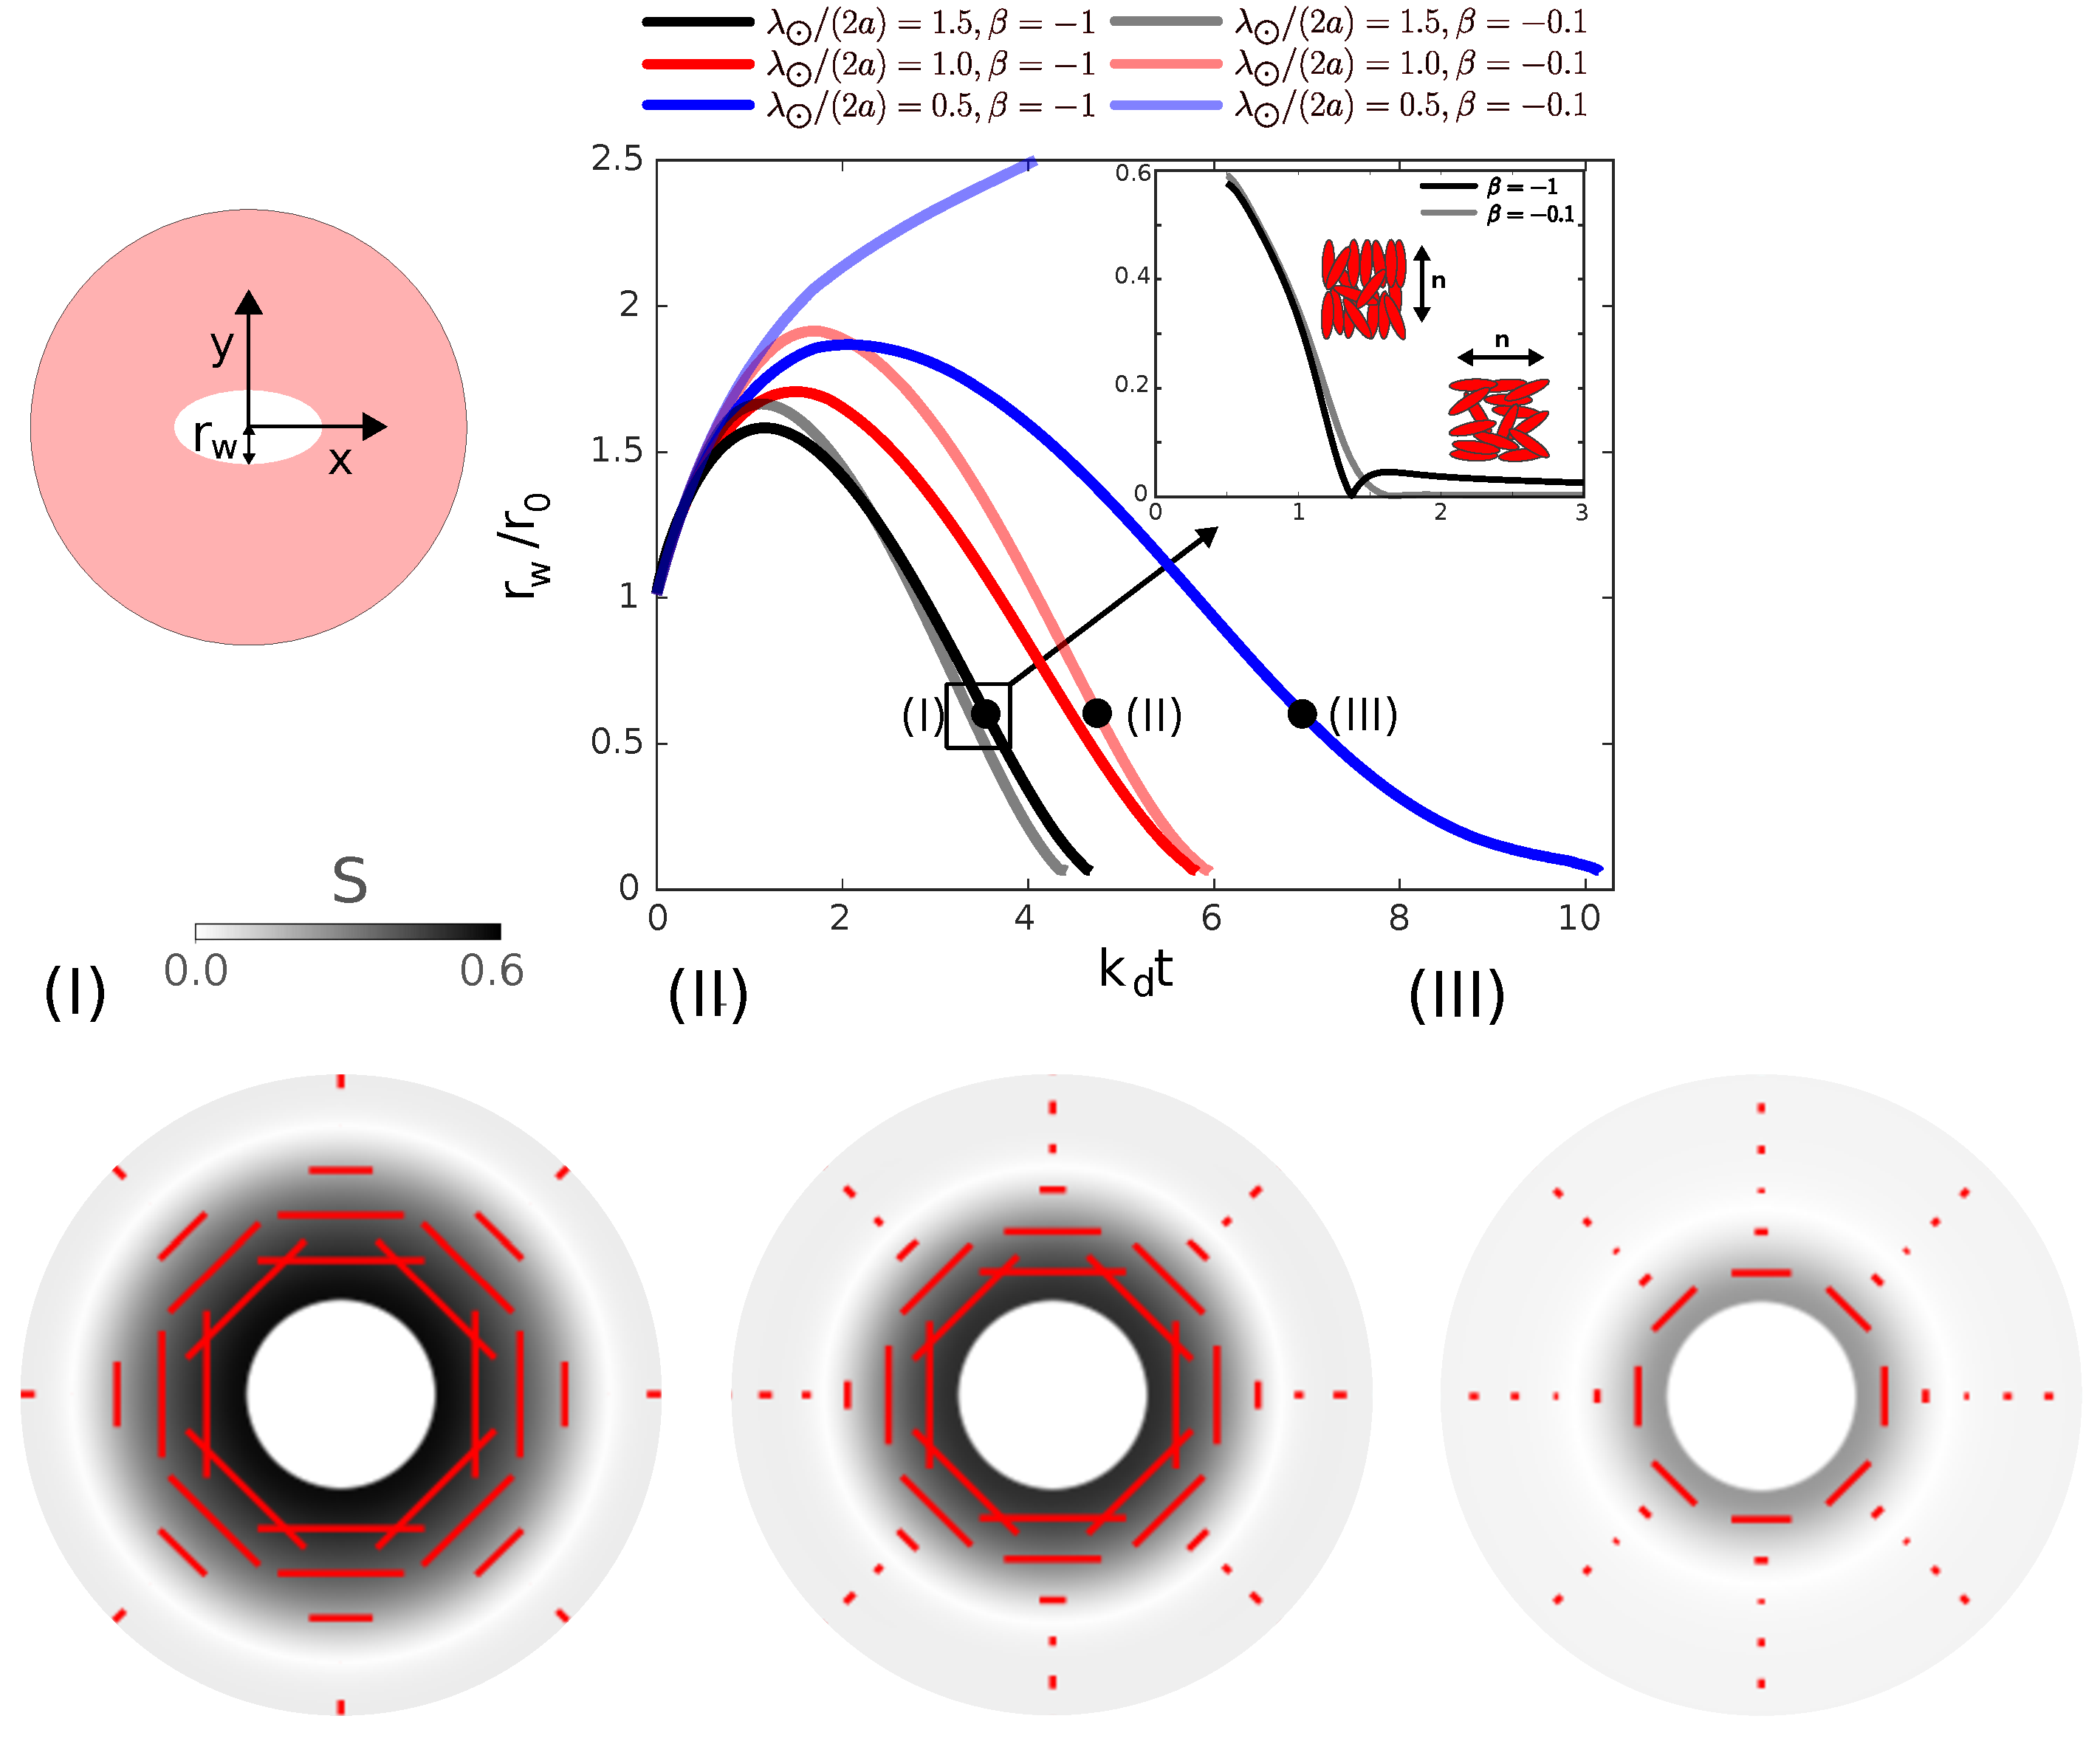
\includegraphics[width=0.85\textwidth]{chap_3_fig_2.pdf}
		\caption{\label{sec_1_chap_3_fig_2}  \textbf{Effect of the flow aligning parameter $\beta$ and nematic activity $\lambda_{\bigodot}$ on the constriction dynamics}. Normalized wound size  $r_w$ as a function of time for different choices of parameters. The snapshots (I-III) show the nematic organization at a given wound size for different $\lambda_{\bigodot}$. Nematic field is represented by a color map for $S$ and by red segments, whose direction indicates the nematic orientation and whose size is proportional to $S$. The size and direction of the red segments indicate the nematic order parameter and average nematic orientation, respectively. }
\end{figure}


\subsection{Defects in a confined colony of spindle-shaped cells}

Elongated spindle-shaped contractile cells such as myoblasts or fibroblasts exhibit long-range nematic order in circular confined dense cultures \cite{duclos2014,guillamat2020} due to their tendency to mutually align parallel with each other \cite{elsdale1968}. Cells confined in these circular domains tend to align parallel or perpendicular to the boundary \cite{guillamat2020}.
Because of this alignment, the net charge of the topological defects in the colony is $+1$, as required by the Poincar\'{e}-Hopf theorem \cite{jubin2009}. This is satisfied by the generation of one or more pairs of topological defects with charge $\pm 1/2$.
%This leads to disruption in the nematic field by self-organization of $\pm 1/2$  topological defects.
Because nematic order controls the anisotropy of active stresses in the cell monolayer, topological defects actively move and may lead to a variety of out-of-equilibrium behaviors. 
Depending on the size of the geometrical confinement with respect to the characteristic lengths of the system, self-organized flows of defects are either absent \cite{duclos2014}, spiral or turbulent-like \cite{norton2018}. 

Here, using the proposed computational framework, we examine the dynamics of a spatially confined dense contractile active nematic system. In this dense cell colony, density variations are arguably small, and hence the density-dependent aspects of our model may not be important. However, we note that an incompressible model for an active liquid crystal may not be pertinent either as convergent/divergent flows are possible due to cell extrusion/proliferation. To simplify the model, we place ourselves in the limit of high turnover rate, for which density is uniform and convergent/divergent flows are allowed. This only leaves us with the coupling between nematic and velocity fields. In order to model the propensity of cells towards mutual alignment, we set the susceptibility parameter such that the initial nematic order is close to $S_0=\sqrt{2|a|/b}=1$. All model parameters are detailed in Table~\ref{modal_parameters}. Furthermore, we impose a boundary condition such that the director field  $\bm{n}|_{\bm{x}=\partial A}$ is fully aligned either tangentially or perpendicularly to the boundary, which corresponds to parallel or homeotropic anchoring  \ref{sec_1_chap_3_fig_3}(a). We enforce that normal velocity to the boundary is zero (impermeable boundary) by using a penalty term in the Rayleighian given as  $\int_{\partial A} K \left|\bm{v} \cdot \bm{N}\right|^2 dl$, where $K$ is the penalty coefficient, but allows cells to slide tangentially along the boundary.

In the first set of tests,  we explore the behavior of a passive nematic system for different ratios of nematic correlation length scale $\ell_p = \sqrt{L/\left(2|a|\right)}$ to the characteristic size of the domain $\ell_0$.  We start with a spatially correlated random initial condition for $\bm{q}$.  Initially, the topological constraints promote a high gradient in nematic orientation which, in turn, nucleate two $+1/2$ defects near the boundary \cite{hardouin2019,giomi2014}. These $+1/2$ defects travel away from the wall into the bulk and reach a quiescent steady-state \cite{giomi2014}. During this process, the system free-energy decreases \ref{sec_1_chap_3_fig_3}(c) and at steady-state, velocities and rate of dissipation vanish. For systems with parallel (homeotropic) boundary conditions, the tips of the $+1/2$ defects point away from (towards) each other (\ref{sec_1_chap_3_fig_3}(b) left inset). The size of the defect cores relative to system size depends on nematic correlation length scale $\ell_p$. As this quantity becomes large, either by increasing the nematic lengthscale or decreasing system size, we expect the two defects to interact and possibly combine into a single $+1$ defect as observed in small-size cell colonies (\ref{sec_1_chap_3_fig_3}(b) right inset). To examine this, we tracked the distance between the two defects, $d$, as a function of  $\ell_p/\ell_0$, finding that beyond a threshold, $d$ abruptly drops close to zero, with configurations resembling vortices or asters depending on boundary conditions, (\ref{sec_1_chap_3_fig_3}(b) right inset). We note, however, than in the absence of activity, $d$ stays finite, and hence the two defects do not strictly become a $+1$ defect, due to the Coulomb repulsion rendering the bound $+1$ defect unstable in absence of activity \cite{thijssen2020, vafa2020}.
\begin{figure}[H]
	\centering
	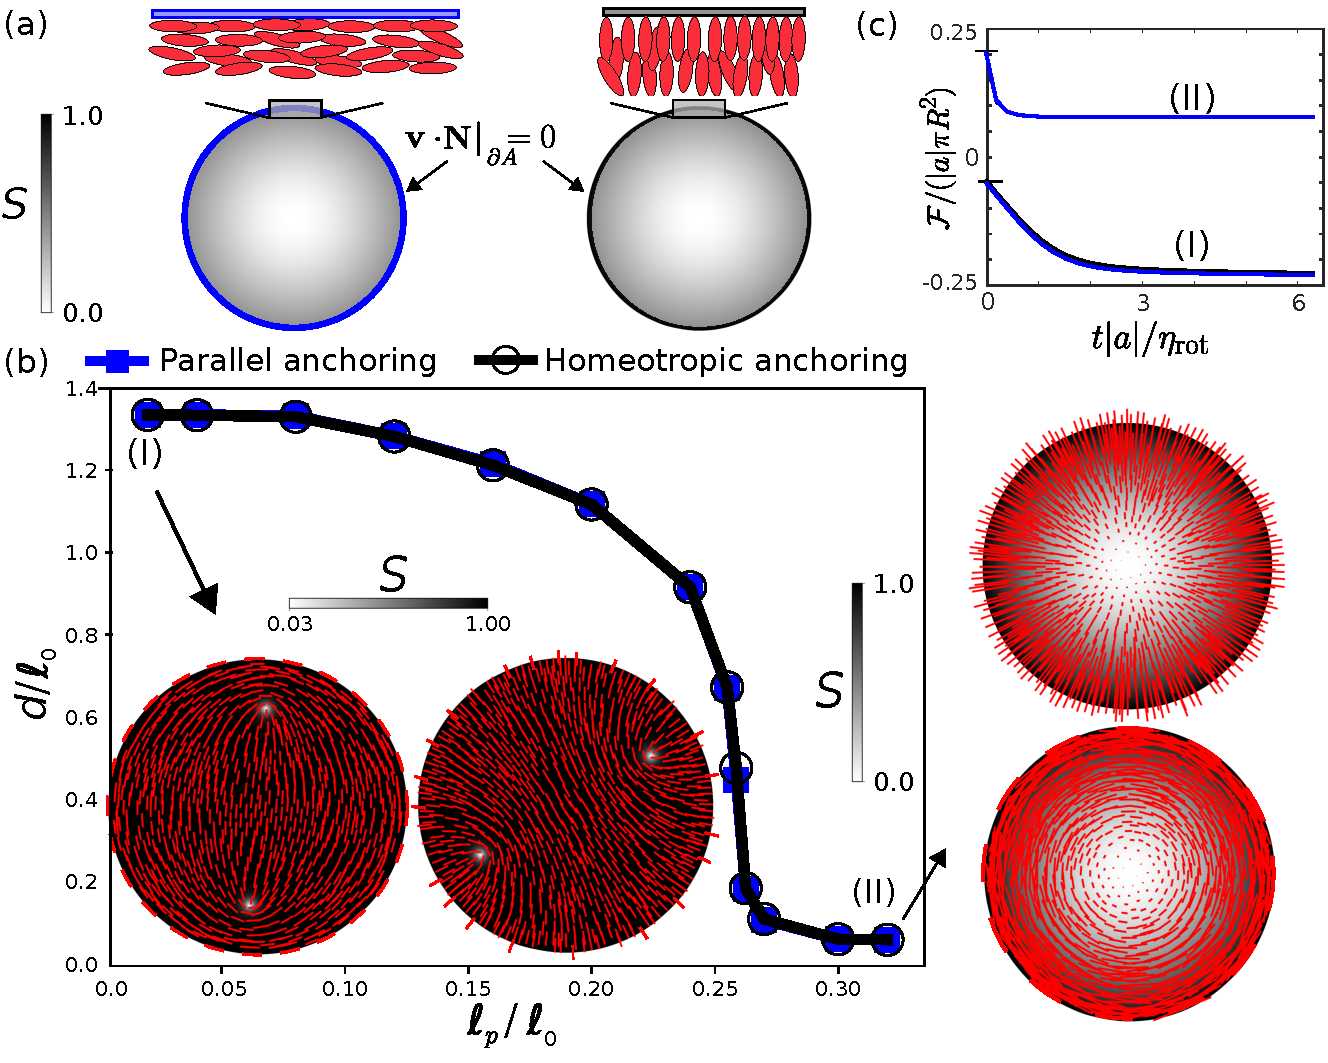
\includegraphics[width=0.75\textwidth]{chap_3_fig_3.pdf}
\caption{\label{sec_1_chap_3_fig_3} \textbf{Effect of nematic correlation length scale $\ell_p$ on the inter-defect distance $d$ in a passive nematic system}. (a) Illustration of nematic and velocity boundary conditions. (b) Inter-defect distance as a function of nematic correlation length scale $\ell_p$ for parallel and homeotropic anchoring conditions, along with selected nematic fields. (c) Monotonically decreasing time-evolution of the Landau free-energy for high and low $\ell_p$ and for both boundary conditions.}
\end{figure}
We next explore the spatiotemporal behavior of defects in a contractile ($\lambda_{\rm aniso} > 0$) active nematic system by examining the  velocity and nematic fields as a function of the active length scale $\ell_a = \sqrt{L/\lambda_{ \rm aniso}}$, given by the ratio of nematic-elastic and active stresses. This active length scale governs fluctuations in both the nematic and velocity fields. We vary this inverse activity parameter at low nematic correlation length scale $\ell_p/\ell_0$ (see Fig.~\ref{sec_1_chap_3_fig_3.5}).  At low activity, we observe that the active contractile stress $\lambda_{\rm aniso} \bm{q}$ leads to new steady-state with a smaller inter-defect distance, Fig.~\ref{sec_1_chap_3_fig_3.5}(b) and left panel of \href{https://github.com/waleedmirzaPhD/movies_thesis.git}{Movie~3.2}, see Appendix~\ref{appendix_3}. More importantly, the steady state of the active system exhibits persistent flows in the nose to tail direction around defects \cite{doostmohammadi2018,ronning2022}, which push these defects by advection of nematic order, Eq.~(\ref{jaumann_detivative_def}). The passive nematic distribution is also distorted slightly by the flow-induced alignment term involving $\beta$.

At a smaller value, $\ell_a/\ell_0 = 0.15$, the two motile $+1/2$ defects move closer together and  towards the wall, with an out-of-equilibrium velocity exhibiting two vortices. After a transient wiggling motion, these to defects stop moving and the system reaches an out-of-equilibrium steady-state,  Fig.~\ref{sec_1_chap_3_fig_3.5}c,d and center panel of \href{https://github.com/waleedmirzaPhD/movies_thesis.git}{Movie~3.2}, see Appendix~\ref{appendix_3}. As we further reduce the ratio $\ell_a/\ell_0$ to $0.1$, the defect distance increases and the two defects rotate in a chiral configuration leading to persistent rotation of the entire system, Fig.~\ref{sec_1_chap_3_fig_3.5}c,d and 
right panel of \href{https://github.com/waleedmirzaPhD/movies_thesis.git}{Movie~3.2}, see Appendix~\ref{appendix_3}. It has been suggested  that the length-scale of such vortex driven by a defect pair is commensurate to $\ell_a$ \cite{chandrakar2020}, and therefore, for lower activity this length-scale is too large for vortices to develop within the domain size. In this regime, the spiral flow suppresses the defect nucleation that might otherwise form through the splay-type hydrodynamic instability \cite{ramaswamy2007, ramaswamy2010}. A similar argument has been made here for bend-type instability for an extensile network of microtubules and  kinesins \cite{opathalage2019}. Upon further lowering the active length scale, $\ell_a/\ell_0 \leq 0.05$ the previously described splay-type hydrodynamic instability emerges \cite{ramaswamy2007, ramaswamy2010}, as shown in Fig.~\ref{sec_1_chap_3_fig_3.5}d (right). In this regime, active stresses overcome the restoring elastic stresses and distort the nematic field to form lines of splay-type disinclination in the bulk and close to the boundary. In turn, these disclination lines destabilize and split into pairs of $\pm 1/2$ defects, which move and annihilate with defects of opposite charge. The persistent generation of disclination lines, their destabilization into point defects, and the motion and annihilation of these defects gives rise to active turbulence, Fig.~\ref{sec_1_chap_3_fig_3.5}(c,d) and  \href{https://github.com/waleedmirzaPhD/movies_thesis.git}{Movie~3.3}, see Appendix~\ref{appendix_3}. At any given time, the system exhibits  more than two defects but the total topological charge is conserved to $+1$.
\begin{figure}[tb]
	\centering
	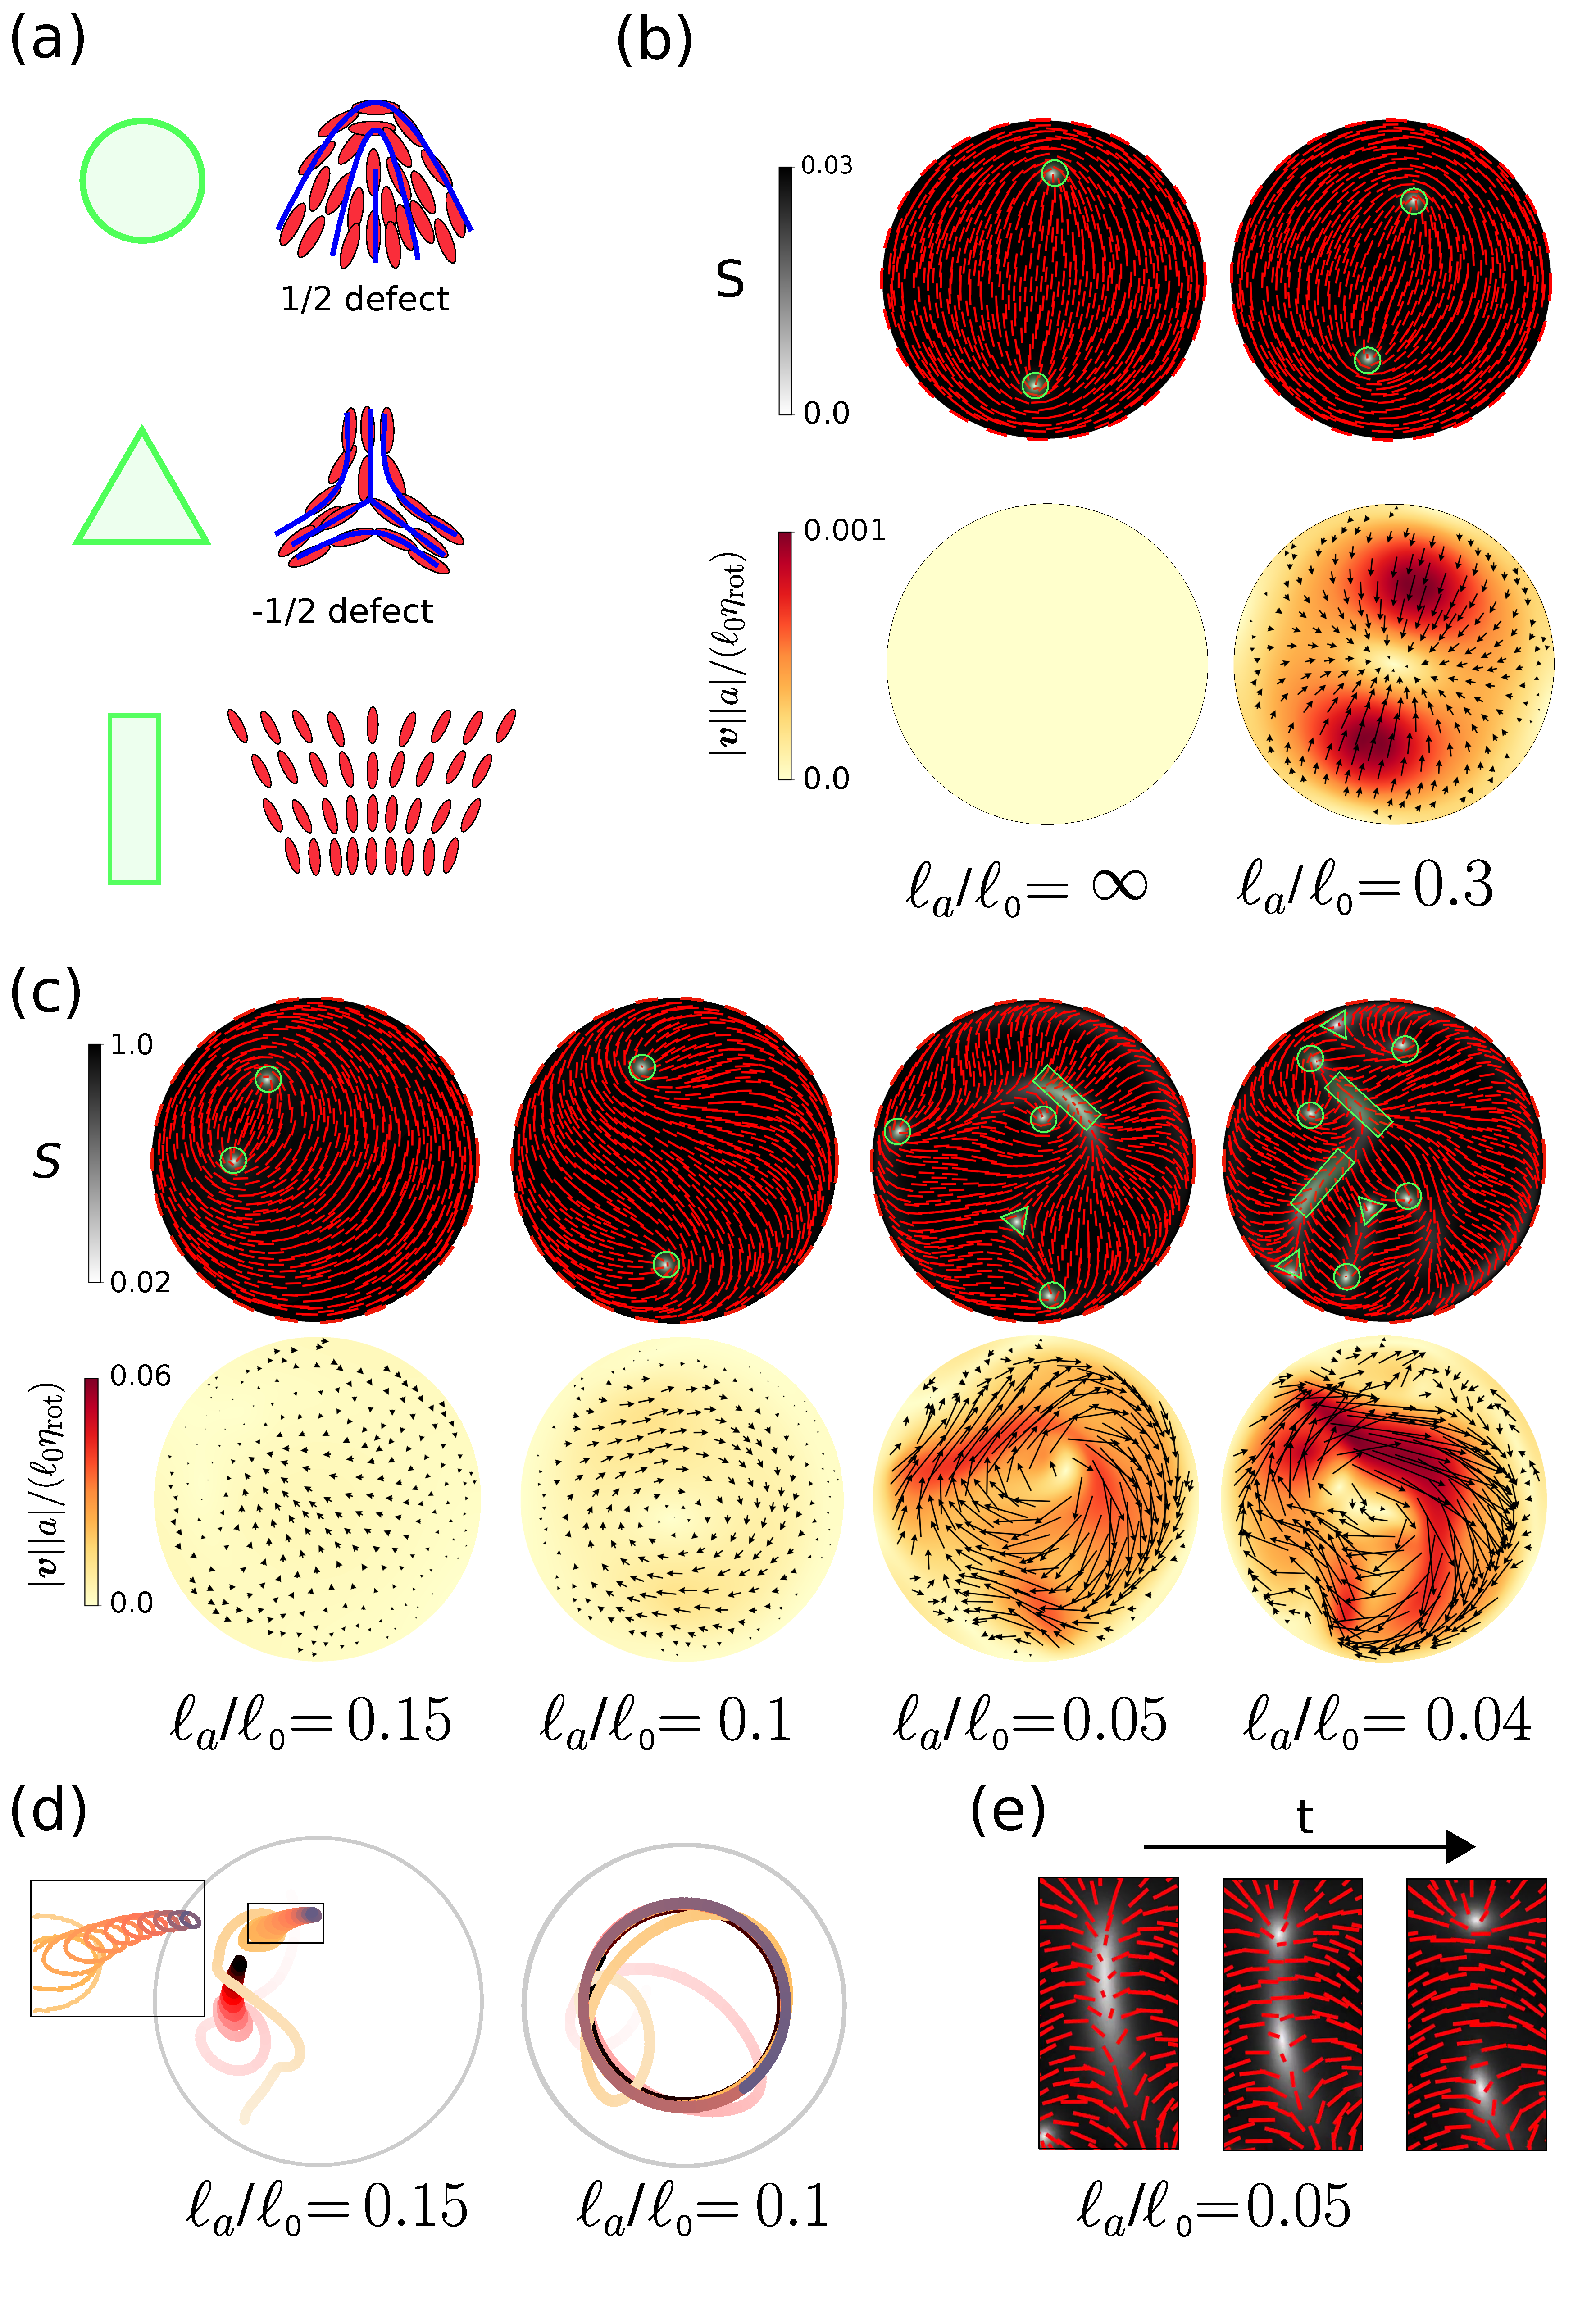
\includegraphics[width=0.62\textwidth]{chap_3_fig_4.pdf}

	\caption{\label{sec_1_chap_3_fig_3.5}  \textbf{Effect of activity on a dense colony of contractile cells under confinement.} (a) Graphical coding of   half integer defects, $\pm \frac{1}{2}$, and of splay bands. (b) Nematic field (top, with segment showing nematic direction and colormap showing order parameter $S$) and velocity and density fields (bottom)  in absence (left) and presence (right) of activity at $\ell_p=0.02$,  \href{https://github.com/waleedmirzaPhD/movies_thesis.git}{Movie~3.2}  (left).	(c) Effect of active nematic length scale on the spatiotemporal distribution of flow, density and nematic fields and $\pm 1/2$ defects at $\ell_p=0.01$,  \href{https://github.com/waleedmirzaPhD/movies_thesis.git}{Movie~3.2}  and \href{https://github.com/waleedmirzaPhD/movies_thesis.git}{Movie~3.3}  (d) Dynamics of the two $+1/2$ defects for $\ell_a/\ell_0=0.15$ and $\ell_a/\ell_0=0.1$. Each defect trajectory becomes darker as time increases. (e) Nucleation of $1/2$ and  $-1/2$ defects from splay bands at $\ell_a/\ell_0=0.05$. }
\end{figure}
In summary, we explored the proposed model in the limit of fast turnover, and hence in the absence of spatio-temporal changes in density, to model a confided cell colony capable of maintaining constant density by rapid division and extrusion. We characterized the passive and active contractile regimes as well as qualitatively compared these behaviors against the literature. In a confided passive nematic system, we observed a canonical spontaneous organization of two $+1/2$ defects with a steady inter-defect distance inversely proportional to the passive nematic length scale $\ell_p  = \sqrt{L/\left(2|a| \right)}$. In the active limit, we observed a diversity of patterns depending on the value of active nematic length-scale $\ell_a= \sqrt{L/\lambda_{\rm aniso}}$.  In general, a gradient in the nematic order in the vicinity of defects generates an active flow, which renders the defects motile. At large values of $\ell_a/\ell_0$, we observe a spiral flow of defects, which turns into a persistent vortical motion in an intermediate range of $\ell_a/\ell_0$. At small values of  $\ell_a/\ell_0$ (high activity), we observe active turbulence in the cell colony characterized by persistent defect nucleation due to splay-type instabilities, motion and annihilation. 

	\section{Summary}


In Chapters~\ref{chap_2} and~\ref{chap_3}, we have proposed a modeling framework for density-dependent active nematic gels based on Onsager's variational formalism. This formalism enables a clear and systematic derivation of otherwise complex equations coupling nematic order, gel velocity and density. We have particularized this framework to develop a specific model, which we have discretized using finite elements and applied to two studies of biological relevance. In the first study, we have explored the role of the self-organization of the actin cytoskeleton during wound repair. We show that a slight overactivity around the wound drives a self-reinforcing flow of the actin network leading to the self-organization of the nematic bundle that efficiently constricts the wound. In a second numerical study, we explore the self-organization of nematic architectures in the limit of high turnover in a constrained colony of contractile cells. Depending on the magnitude of the activity, the topological defects required by boundary conditions either reach a steady state or exhibit highly dynamical flows as well as active turbulence.

%Our framework provides a basis to explore a large variety of active nematic systems. Although here we have focused on simple cases where the nematic architectures are self-organized in a contractile network due to slight overactivity of myosin in the cytoskeleton or due to boundary conditions in a colony of contractile cells, our framework can be applied to understand the diversity of nematic architectures in actomyosin networks \cite{mirza2022}, including bundles  \cite{tojkander2015,jalal2019, vignaud2021}, asters \cite{xia2019}, and tactoids \cite{weirich2017,weirich2019}. If suitably extended to curved and time-evolving surface domains \cite{mirza2023}, the framework presented here can help us examine the interaction between nematodynamics and reshaping during cytokinesis \cite{mayer2010} or hydra morphogenesis \cite{maroudas2021}.


\newpage
